\documentclass[tikz,border=5pt]{standalone}
\usepackage{graphicx} % Required for inserting images




% ====== Preamble requirements (add once) ======
\usepackage{tikz}
\usetikzlibrary{arrows.meta,positioning,shapes.geometric,shapes.misc,fit,calc}

\title{RandD-graphs}
\author{romain.ryckebusch }
\date{December 2025}

\begin{document}


% ====== Figure: Full continuity algorithm (flowchart) ======
\begin{figure}[h]
\centering
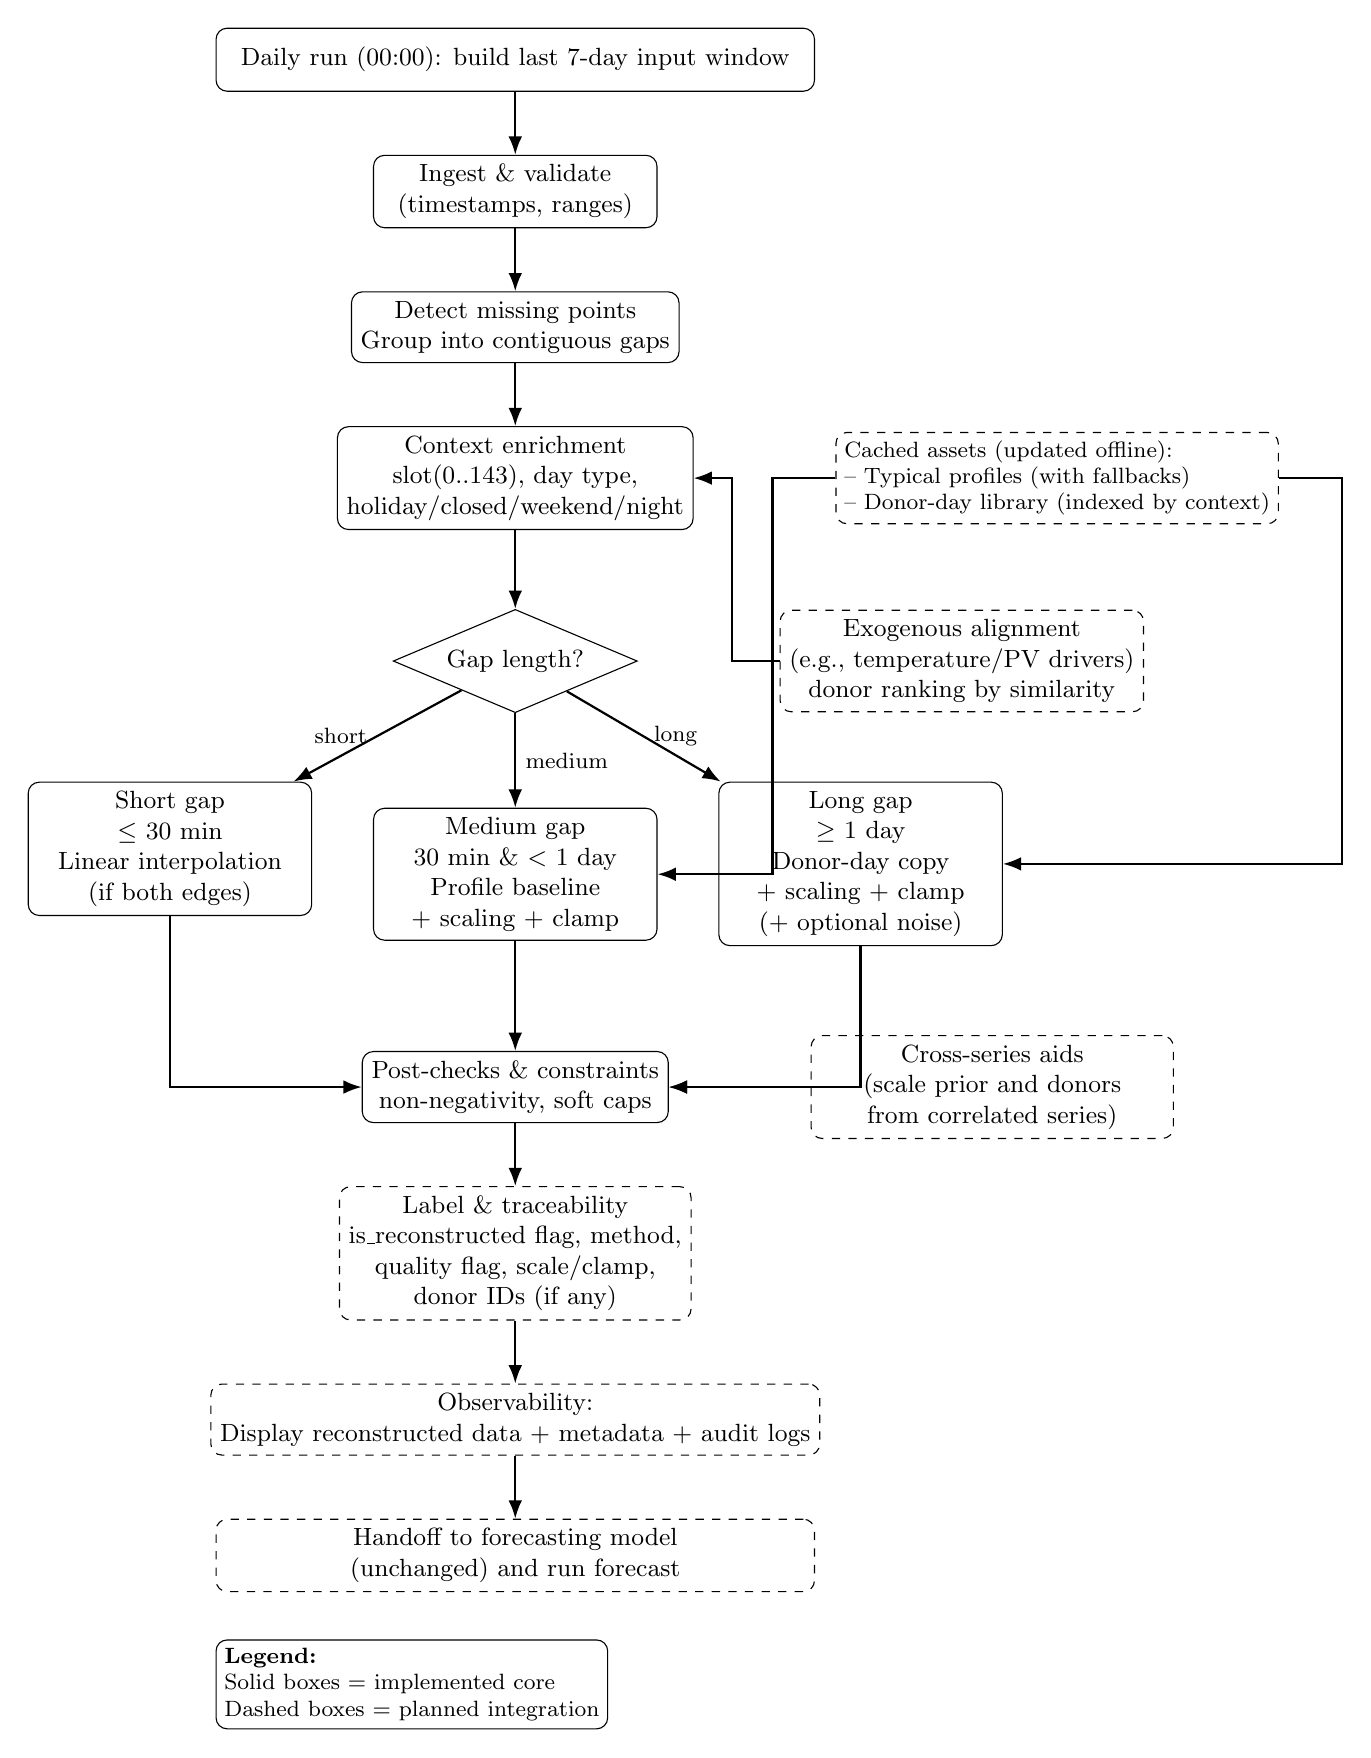
\begin{tikzpicture}[
  font=\small,
  node distance=8mm and 12mm,
  box/.style={draw, rounded corners, align=center, minimum width=3.6cm, minimum height=8mm},
  wide/.style={draw, rounded corners, align=center, minimum width=7.6cm, minimum height=8mm},
  decision/.style={draw, diamond, aspect=2, align=center, inner sep=1.5pt, minimum width=3.1cm, minimum height=9mm},
  note/.style={draw, rounded corners, align=left, inner sep=3pt, font=\footnotesize},
  planned/.style={draw, dashed, rounded corners, align=center},
  arrow/.style={-Latex, thick}
]

% Main pipeline
\node[wide] (start) {Daily run (00:00): build last 7-day input window};
\node[box, below=of start] (ingest) {Ingest \& validate\\(timestamps, ranges)};
\node[box, below=of ingest] (gaps) {Detect missing points\\Group into contiguous gaps};
\node[box, below=of gaps] (context) {Context enrichment\\slot(0..143), day type,\\holiday/closed/weekend/night};

\node[decision, below=10mm of context] (len) {Gap length?};

\node[box, below left=12mm and 18mm of len] (short) {Short gap\\$\le$ 30 min\\Linear interpolation\\(if both edges)};
\node[box, below=12mm of len] (med) {Medium gap\\30 min \& $<$ 1 day\\Profile baseline\\+ scaling + clamp};
\node[box, below right=12mm and 18mm of len] (long) {Long gap\\$\ge$ 1 day\\Donor-day copy\\+ scaling + clamp\\(+ optional noise)};

\node[box, below=14mm of med] (post) {Post-checks \& constraints\\non-negativity, soft caps};
\node[planned, box, below=of post] (label) {Label \& traceability\\is\_reconstructed flag, method,\\quality flag, scale/clamp,\\donor IDs (if any)};
\node[planned, wide, below=of label] (store) {Observability:\\Display reconstructed data + metadata + audit logs};
\node[planned, wide, below=of store] (forecast) {Handoff to forecasting model\\(unchanged) and run forecast};

% Side caches / assets
\node[planned, note, right=18mm of context] (assets) {Cached assets (updated offline):\\
-- Typical profiles (with fallbacks)\\
-- Donor-day library (indexed by context)};
\draw[arrow] (assets.west) -- ++(-8mm,0) |- (med.east);
\draw[arrow] (assets.east) -- ++(+8mm,0) |- (long.east);

% Planned integrations
\node[planned, right=18mm of len, minimum width=4.6cm, minimum height=1.2cm] (exo) {Exogenous alignment\\(e.g., temperature/PV drivers)\\donor ranking by similarity};
\draw[arrow] (exo.west) -- ++(-6mm,0) |- (context.east);

\node[planned, right=18mm of post, minimum width=4.6cm, minimum height=1.0cm] (multi) {Cross-series aids\\(scale prior and donors\\from correlated series)};
\draw[arrow] (multi.west) -- ++(-6mm,0) |- (post.east);

% Connections
\draw[arrow] (start) -- (ingest);
\draw[arrow] (ingest) -- (gaps);
\draw[arrow] (gaps) -- (context);
\draw[arrow] (context) -- (len);

\draw[arrow] (len) -- node[midway, left, font=\footnotesize] {short} (short);
\draw[arrow] (len) -- node[midway, right, font=\footnotesize] {medium} (med);
\draw[arrow] (len) -- node[midway, right, font=\footnotesize] {long} (long);

\draw[arrow] (short) |- (post);
\draw[arrow] (med) -- (post);
\draw[arrow] (long) |- (post);

\draw[arrow] (post) -- (label);
\draw[arrow] (label) -- (store);
\draw[arrow] (store) -- (forecast);

% Legend
\node[note, below left=6mm and 0mm of forecast, anchor=north west] (legend) {
\textbf{Legend:}\\
Solid boxes = implemented core\\
Dashed boxes = planned integration
};

\end{tikzpicture}
\caption{Continuity / reconstruction layer ensuring a complete 7-day window at midnight.}
\end{figure}


\end{document}
